\capitulo{5}{Aspectos relevantes del desarrollo del proyecto}

\begin{comment}
Este apartado pretende recoger los aspectos más interesantes del desarrollo del proyecto, comentados por los autores del mismo.
Debe incluir desde la exposición del ciclo de vida utilizado, hasta los detalles de mayor relevancia de las fases de análisis, diseño e implementación.
Se busca que no sea una mera operación de copiar y pegar diagramas y extractos del código fuente, sino que realmente se justifiquen los caminos de solución que se han tomado, especialmente aquellos que no sean triviales.
Puede ser el lugar más adecuado para documentar los aspectos más interesantes del diseño y de la implementación, con un mayor hincapié en aspectos tales como el tipo de arquitectura elegido, los índices de las tablas de la base de datos, normalización y desnormalización, distribución en ficheros3, reglas de negocio dentro de las bases de datos (EDVHV GH GDWRV DFWLYDV), aspectos de desarrollo relacionados con el WWW...
Este apartado, debe convertirse en el resumen de la experiencia práctica del proyecto, y por sí mismo justifica que la memoria se convierta en un documento útil, fuente de referencia para los autores, los tutores y futuros alumnos.
\end{comment}

\section{Procesamiento de imagenes}

Como primera aproximación al problema que nos concierne hemos escogido el procesamiento de imagenes mediante la librería Scikit-image para Python. Mediante esta herramienta trataremos de dar solución a nuestro problema siguiendo los siguientes pasos:

\begin{enumerate}[1.]
  \item Convertimos la imagen a escala de grises
  \item Segmentamos los objetos del fondo de la imagen
  \item Obtenemos los distintos objetos de la imagen
\end{enumerate}

\subsection{Convertimos la imagen a escala de grises}

La conversión de la imagen original (RGB) a escala de grises viene motivada porque para poder segmentar los objetos del fondo de la imagen mediante el método de \textit{Thresholding} solo se puede partir de una imagen en escala de grises.

\begin{figure}
	\centering
	\begin{subfigure}[b]{0.45\textwidth}
        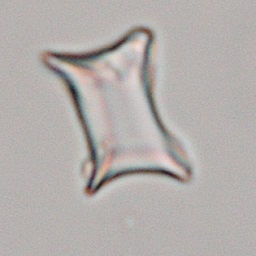
\includegraphics[width=\textwidth]{2}
        \caption{Original}
    \end{subfigure}
    \begin{subfigure}[b]{0.45\textwidth}
        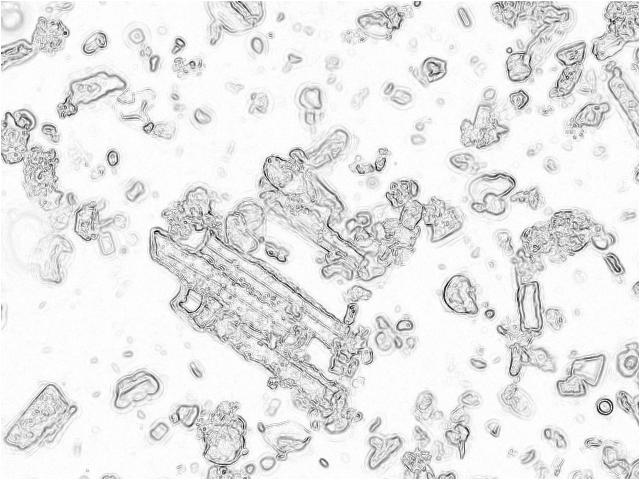
\includegraphics[width=\textwidth]{grayscale_image}
        \caption{Imagen en escala de grises}
    \end{subfigure}
\end{figure}

\subsection{Segmentamos los objetos del fondo de la imagen}

Una vez tenemos la imagen en escala de grises procedemos a transformar nuestra imagen en una imagen en blanco y negro o binarizada. Los motivos por los que binarizamos la imagen es para obtener una imagen que sea más significativa para nosotros y además este simplificada, para facilitarnos su procesamiento.

Scikit nos propociona distintos métodos mediante los cuales podemos segmentar una imagen. A continuación vamos a ver el resultado aplicando distintos métodos, los cuales se van indicando en cada una de las figuras:

\begin{figure}
	\centering
	\begin{subfigure}[b]{0.45\textwidth}
        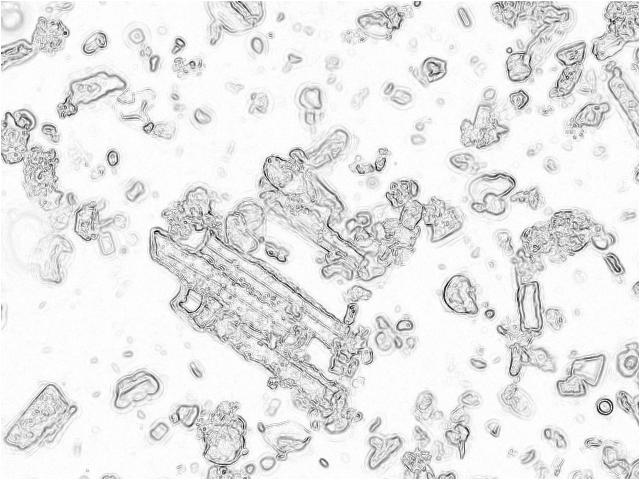
\includegraphics[width=\textwidth]{grayscale_image}
        \caption{Imagen en escala de grises}
    \end{subfigure}
    \begin{subfigure}[b]{0.45\textwidth}
        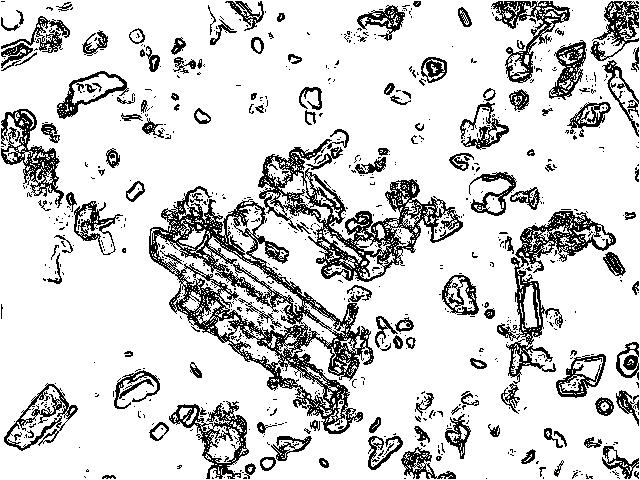
\includegraphics[width=\textwidth]{otsu_threshold_image}
        \caption{Método de Otsu}
    \end{subfigure}
    \begin{subfigure}[b]{0.45\textwidth}
        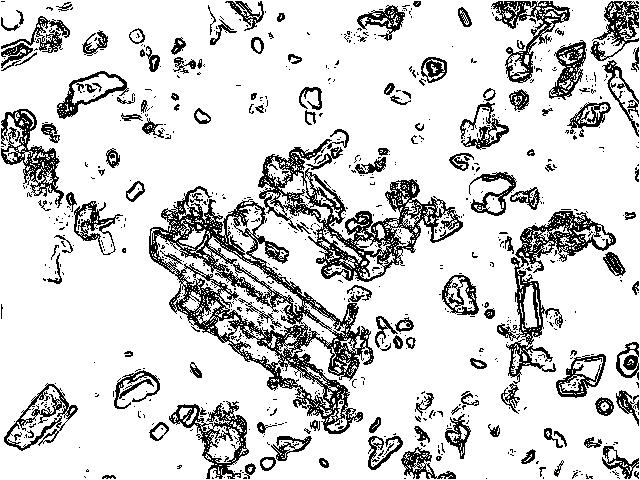
\includegraphics[width=\textwidth]{otsu_threshold_image}
        \caption{Método de Otsu}
    \end{subfigure}
    \begin{subfigure}[b]{0.45\textwidth}
        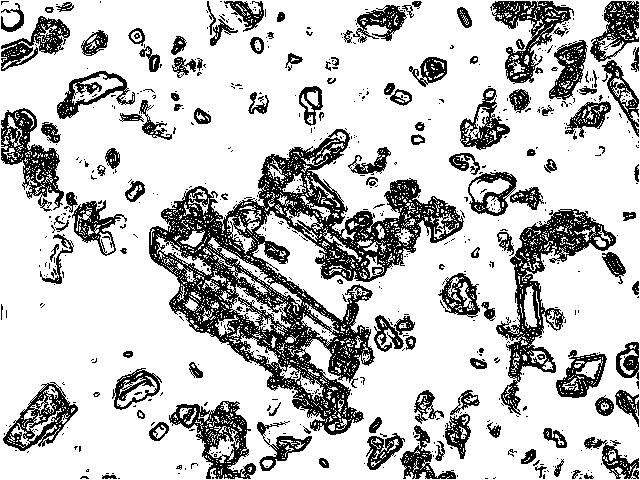
\includegraphics[width=\textwidth]{yen_image}
        \caption{Método de Yen}
    \end{subfigure}
    \begin{subfigure}[b]{0.45\textwidth}
        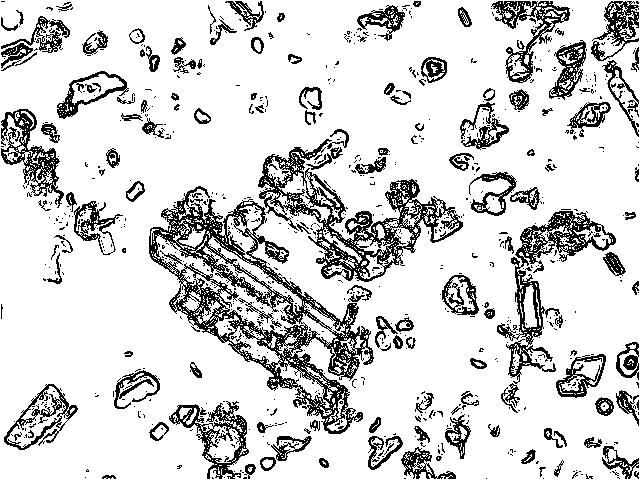
\includegraphics[width=\textwidth]{li_thresholded_image}
        \caption{Método de Li}
    \end{subfigure}
    \begin{subfigure}[b]{0.45\textwidth}
        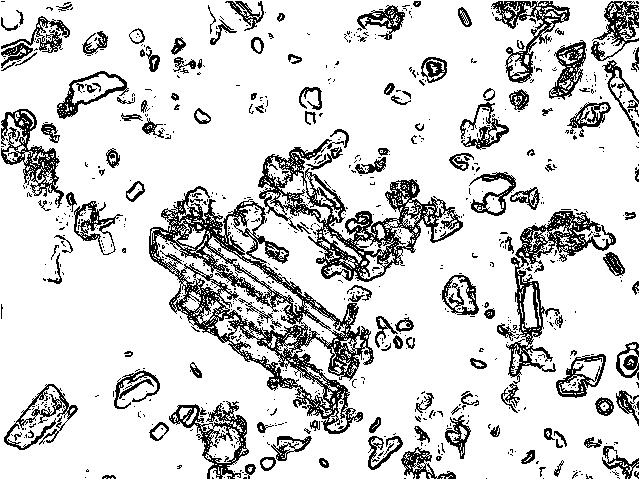
\includegraphics[width=\textwidth]{isodata_thresholded_image}
        \caption{Método de ISODATA}    
    \end{subfigure}
    \begin{subfigure}[b]{0.45\textwidth}
        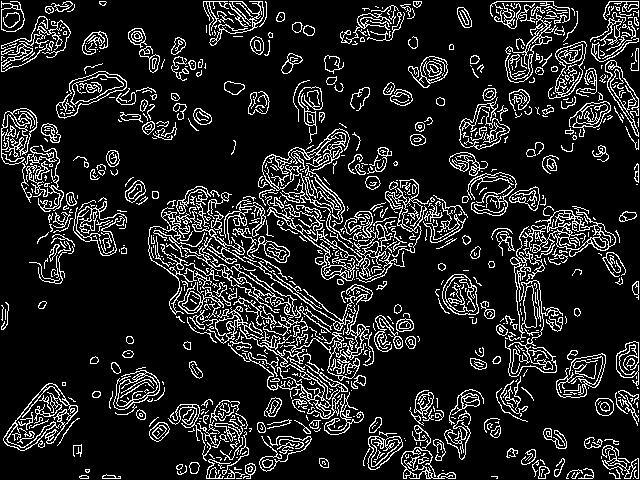
\includegraphics[width=\textwidth]{edge_based_image}
        \caption{Método basado en bordes}    
    \end{subfigure}
    \begin{subfigure}[b]{0.45\textwidth}
        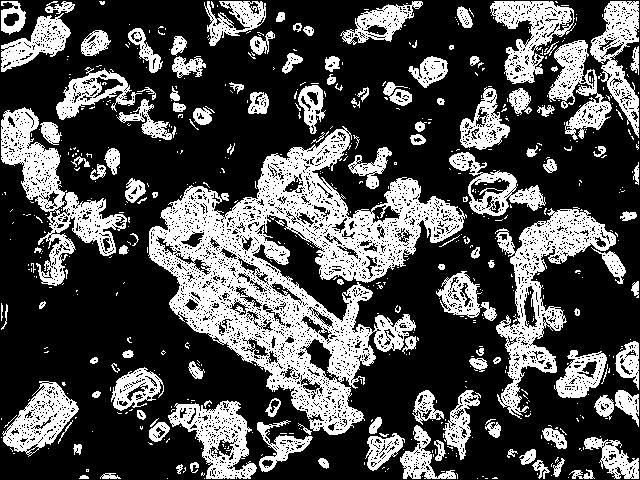
\includegraphics[width=\textwidth]{adaptive_thresholded_image_5}
        \caption{Método adaptativo}    
    \end{subfigure}
\end{figure} 

\subsection{Obtenemos los distintos objetos de la imagen}
Después de tener la imagen binarizada de la forma más apropiada posible probamos a segmentar los distintos objetos de nuestra imagen.

\subsection{Transformación divisoria}
Transformación divisoria, o en ingles \textit{Watershed segmentation}, es un algoritmo clásico en la segmentación de objetos en una imagen.

Durante las primeras pruebas la segmentación más interesante hasta el momento ha sido la que se muestra a continuación a partir del \textit{Watershed segmentation} con marcado. Más allá de esta segmentación no se ha conseguido nada mejor.

\begin{figure}
	\centering
	\begin{subfigure}[b]{0.45\textwidth}
        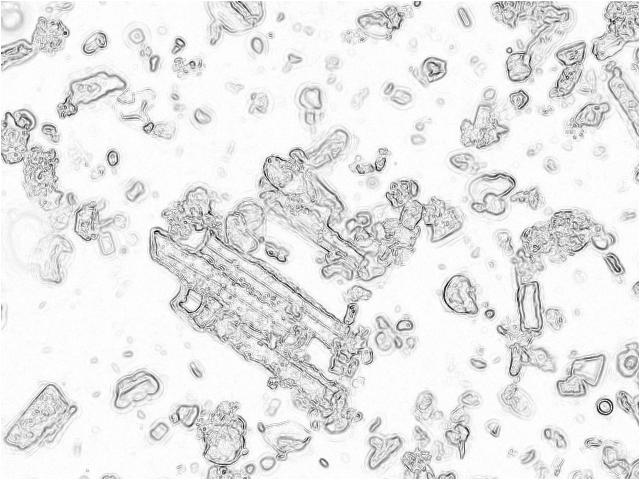
\includegraphics[width=\textwidth]{grayscale_image}
        \caption{Imagen en escala de grises}
    \end{subfigure}
    \begin{subfigure}[b]{0.45\textwidth}
        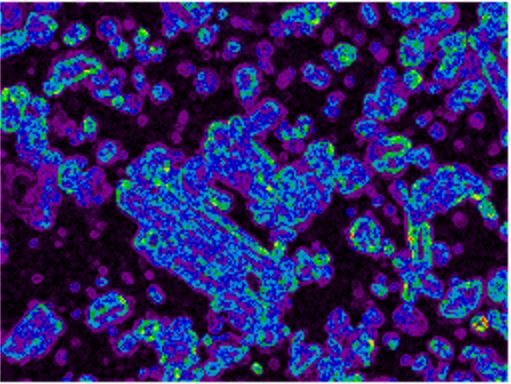
\includegraphics[width=\textwidth]{local_gradient_gimp}
        \caption{Gradiente de la imagen}
    \end{subfigure}
    \begin{subfigure}[b]{0.45\textwidth}
        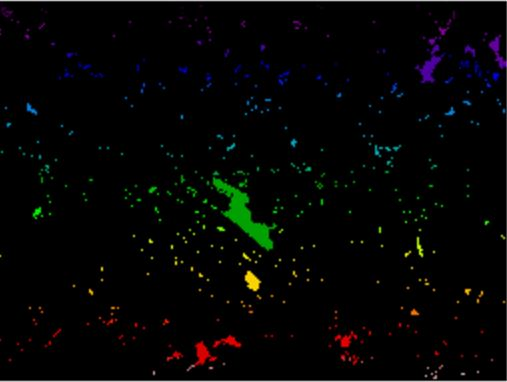
\includegraphics[width=\textwidth]{markers_gimp}
        \caption{Marcadores}
    \end{subfigure}
        \begin{subfigure}[b]{0.45\textwidth}
        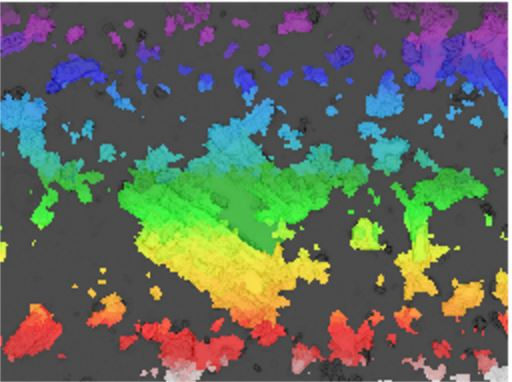
\includegraphics[width=\textwidth]{segmented}
        \caption{Imagen segmentada}
    \end{subfigure}
\end{figure} 	

\section{Clasificadores}
La aproximación mediante procesamiento de imágenes no parece la más adecuada visto los resultados obtenidos. Por ello vamos a realizar el estudio sobre una segunda aproximación  mediante máquinas de vector soporte, para la tarea de clasificación, junto a Histogramas de los gradientes orientados, la cual es una técnica para la extracción automática de características.

El procedimiento para obtener el clasificador es el siguiente:

\begin{enumerate}[1.]
  \item Crear un conjunto de entrenamiento de imágenes de caras que supongan positivos.
  \item Crear un conjunto de entrenamiento de imágenes de no-caras que supongan falsos-positivos.
  \item Extraer las características de HoG del conjunto de entrenamiento.
  \item Entrenar el clasificador SVM.
\end{enumerate}

 Finalizado el entrenamiento de la SVM, ya tenemos nuestro clasificador listo para enviarle nuevas imágenes y que sean clasificadas.
 
\subsection{Reconocimiento de imágenes en nuevas imágenes}
Para el reconocimiento de objetos en nuevas imágenes deberemos de llevar a cabo los 2 siguientes pasos:

\begin{enumerate}[1.]
  \item Pasar una ventana por toda la imagen, comprobando si la ventana contiene un objeto.
  \item Si existe solapamiento en la detección del objeto, muy común en el uso de este tipo de clasificadores, se deben de combinar dichos solapamientos en uno único.
\end{enumerate}

En cuanto al primer paso, lo único a lo que nos referimos es que para el procesado de nuevas imágenes, una ventana del mismo tamaño que las imágenes con las que ha sido entrenado el clasificador recorre toda la imagen comprobando si cada una de las porciones de la imagen contiene el objeto deseado.

El problema de este método es que nos reconocerá muchos más objetos de lo que realmente tenemos en la imagen. Debido a que la ventana recorre linealmente la imagen, por lo que reconocerá el mismo objeto varias veces en ventanas muy próximas, como podemos deducir que es totalmente lógico, ya que esas ventanas serán muy similares y por lo tanto tendrán unas características muy parecidas entre sí. Por ello se aplica el segundo paso sobre los objetos reconocidos, que es la eliminación del solapamiento de objetos mediante la técnica de \textit{Non-Maximum suprresion}.

Como previa experimentación con esta metodología, vamos a entrenar el clasificador para el reconocimiento de caras. Y en función de la efectividad del método sobre las caras tomaremos una serie de conclusiones sobre las que decidamos si llevar a cabo esta solución de nuestro problema.

\subsection{Aplicación sobre el reconocimiento de caras}

A modo de aclaración de las explicaciones anteriores y para que podamos apreciar los resultados, vamos a ver algunas de las imágenes resultantes del clasificador.

Como explicábamos anteriormente, una vez tenemos nuestro clasificador le enviamos una nueva imagen, como podría ser la presentada en la figura \ref{subfig:family}. A partir de esta imagen el clasificador nos permitirá obtener las ventanas en las que detecta una cara, como vemos en la figura \ref{subfig:family_labeled}. Podemos apreciar que existe más de una ventana alrededor de cada cara. Y finalmente, tras aplicar el método \textit{Non-Maximum suprresion} obtenemos el resultado final mostrado en la figura \ref{subfig:family_labeled_nms}.

\begin{figure}
	\centering
	\begin{subfigure}[b]{0.45\textwidth}
        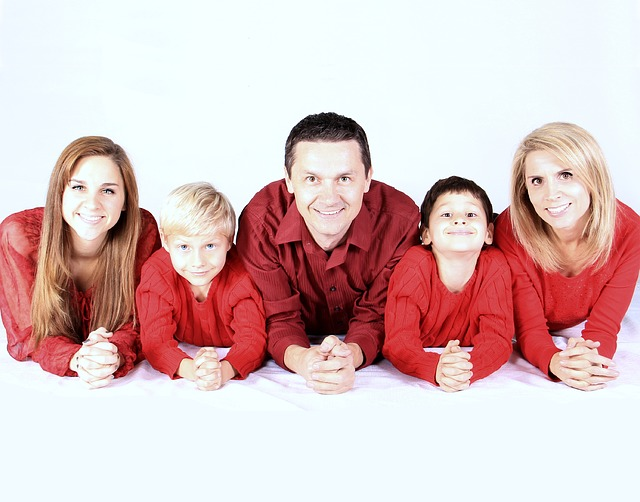
\includegraphics[width=\textwidth]{family}
        \caption{Imagen original}
        \label{subfig:family}
    \end{subfigure}
    \begin{subfigure}[b]{0.45\textwidth}
        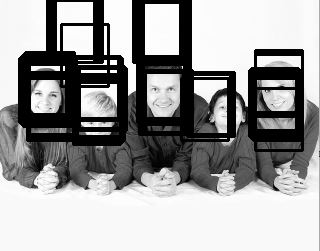
\includegraphics[width=\textwidth]{family_labeled}
        \caption{Imagen después de aplicarla nuestro clasificador}
        \label{subfig:family_labeled}
    \end{subfigure}
    \begin{subfigure}[b]{0.45\textwidth}
        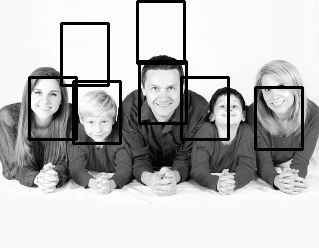
\includegraphics[width=\textwidth]{family_labeled_nms}
        \caption{Imagen tras aplicarla \textit{Non-Maximum suprresion}}
         \label{subfig:family_labeled_nms}
    \end{subfigure}
\end{figure}